\documentclass[9pt,aspectratio=43]{beamer}
\usepackage{tikz}
\usetheme{Boadilla}
\setbeamertemplate{navigation symbols}{}
\title{Message passing: experiments and bounds}
\subtitle{Generated interaction study}
\author{Research group}
\date{}
\year=2026\month=11\day=5
\newcommand{\fuzzlayerA}[1]{\textrm{#1}}
\newcommand{\fuzzterm}[1]{\fuzzlayerA{#1}}
\newcommand{\fuzzpair}[2]{\fuzzterm{#1}: #2}
\newcommand{\fuzzunit}{Hz}
\let\fuzzoriginalunit\fuzzunit
\newcommand{\fuzzcoefficient}{3}
\newcommand{\fuzzscale}[2][\fuzzcoefficient]{#1\,#2}
\definecolor{fuzzpaint}{RGB}{255,0,255}
\definecolor{fuzzsecond}{RGB}{18,137,67}
\tikzset{fuzzvertex/.style={draw,rounded corners=1pt,fill=blue!10,inner sep=1pt,minimum width=.35cm,minimum height=.25cm}}
\begin{document}
\section{Message passing}
\begin{frame}[t,shrink=5]{Message passing}{Composed dependencies}
\fuzzpair{Experiment}{Timing: 12\fuzzunit; estimate $\fuzzscale{x}+\fuzzscale[2]{y}$.}\par
{\renewcommand{\fuzzunit}{ticks}\let\fuzzterm\textbf\fuzzpair{LocalScope}{Timing: 7\fuzzunit.}\par}
\fuzzpair{RestoredScope}{Timing: 11\fuzzunit.}\par
\begin{columns}[onlytextwidth,c]
\begin{column}{0.46\textwidth}
\begin{itemize}
\item<1-> \alt<1-2>{\textbf{The final diagram} records the order in which information crosses the partition. A narrow column can change line breaking even when the underlying expression is unchanged. The estimate is $x_i+x_{i+1}$.}{Alternative estimate $x_0$.}
\item<2-> 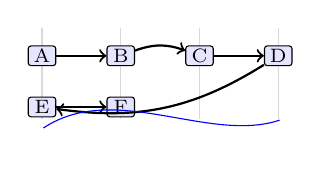
\begin{tikzpicture}[font=\scriptsize]
\begin{scope}[scale=1,rotate=0]

\foreach \x in {0,1,2,3} {\draw[gray!30] (\x*1.000,-.8)--(\x*1.000,.35);}
\node[fuzzvertex] (g5n0) at (0.000,0) {A};
\node[fuzzvertex] (g5n1) at (1.000,0) {B};
\node[fuzzvertex] (g5n2) at (2.000,0) {C};
\node[fuzzvertex] (g5n3) at (3.000,0) {D};
\node[fuzzvertex] (g5n4) at (0.000,-0.65) {E};
\node[fuzzvertex] (g5n5) at (1.000,-0.65) {F};
\begin{scope}[xshift=.5pt,yshift=-.5pt]
\draw<2->[->,thick] (g5n0) -- (g5n1);
\draw<2->[->,thick] (g5n1) to[bend left=20] (g5n2);
\draw<2->[->,thick] (g5n2) -- (g5n3);
\draw<2->[->,thick] (g5n3) to[bend left=20] (g5n4);
\draw<2->[->,thick] (g5n4) -- (g5n5);
\draw[blue] (0,-.9) .. controls (0.900,-.3) and (2.100,-1.1) .. (3.000,-.8);
\end{scope}
\end{scope}
\end{tikzpicture}
\par
\begin{description}
\item<1->[Stage 1] 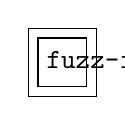
\begin{tikzpicture}\node[draw] {\includegraphics[draft,width=18pt]{fuzz-images/pattern.png}};\end{tikzpicture}
\end{description}
\end{itemize}
\end{column}
\begin{column}{0.50\textwidth}
\begin{description}
\item[Stage 1] {\scriptsize\color{black}\raggedright
\visible<1-2>{\[\begin{aligned}a+b&=c\\ d-e&=f\end{aligned}\]}\par}
\item[Stage 2] \begin{tabular}{lrr}Method&Cost&Error\\\hline
Local0&0&1\\
Local1&3&2\\
Local2&3&19\\
Cached3&13&16\\
\end{tabular}
\par
\textit{A narrow column} can change line breaking even when the underlying expression is unchanged. The next pass must preserve the boundary conditions while revisiting dependent values. The estimate is $\sum_{i=1}^{n}x_i$.
\par
\textrm{A narrow column} can change line breaking even when the underlying expression is unchanged.  The estimate is $\sum_{i=1}^{n}x_i$.
\item[Stage 3] \begin{columns}[onlytextwidth,b]
\begin{column}{0.38\textwidth}
Before 
\includegraphics[page=2,trim=2 1 3 2,clip,width=20pt]{fuzz-images/pages.pdf} after.
\end{column}
\begin{column}{0.58\textwidth}
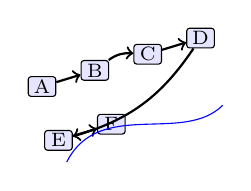
\begin{tikzpicture}[font=\scriptsize]
\begin{scope}[scale=1.1,rotate=17]


\node[fuzzvertex] (g18n0) at (0.000,0) {A};
\node[fuzzvertex] (g18n1) at (0.638,0) {B};
\node[fuzzvertex] (g18n2) at (1.276,0) {C};
\node[fuzzvertex] (g18n3) at (1.914,0) {D};
\node[fuzzvertex] (g18n4) at (0.000,-0.65) {E};
\node[fuzzvertex] (g18n5) at (0.638,-0.65) {F};
\begin{scope}[xshift=.5pt,yshift=-.5pt]
\draw<2->[->,thick] (g18n0) -- (g18n1);
\draw<2->[->,thick] (g18n1) to[bend left=20] (g18n2);
\draw<2->[->,thick] (g18n2) -- (g18n3);
\draw<2->[->,thick] (g18n3) to[bend left=20] (g18n4);
\draw<2->[->,thick] (g18n4) -- (g18n5);
\draw[blue] (0,-.9) .. controls (0.574,-.3) and (1.340,-1.1) .. (1.914,-.8);
\end{scope}
\end{scope}
\end{tikzpicture}
\end{column}
\end{columns}
\end{description}
\end{column}
\end{columns}
\par 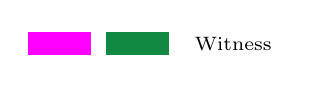
\begin{tikzpicture}[font=\scriptsize]
\fill<2-3>[fuzzpaint] (0,0) rectangle (.8,.3);
\fill<3->[fuzzsecond] (1,0) rectangle (1.8,.3);
\node[anchor=west] at (2,0.15) {Witness};
\end{tikzpicture}
\only<4>{}
\end{frame}
\renewcommand{\fuzzunit}{us}
\renewcommand{\fuzzcoefficient}{2}
\renewcommand{\fuzzterm}[1]{{\textit{#1}}}
\section{Message passing}
\begin{frame}[t]{Cache invalidation}
\fuzzpair{MacroStageB}{Timing: 12\fuzzunit, retained: 9\fuzzoriginalunit.}\par
{\renewcommand{\fuzzunit}{local}\fuzzpair{FrameLocal}{Timing: 5\fuzzunit.}\par}
\fuzzpair{FrameRestored}{Timing: 8\fuzzunit; estimate $\fuzzscale{x}$.}\par
\begin{columns}[T]\begin{column}{.46\textwidth}The next pass must preserve the boundary conditions while revisiting dependent values.\end{column}\begin{column}{.46\textwidth}\begin{itemize}\item Input state\item Updated state\end{itemize}\end{column}\end{columns}
\end{frame}
\renewcommand{\fuzzunit}{min}
\renewcommand{\fuzzcoefficient}{3}
\renewcommand{\fuzzterm}[1]{{\textbf{#1}}}
\section{Message passing}
\begin{frame}[t]{Iterative refinement}
\fuzzpair{MacroStageC}{Timing: 12\fuzzunit, retained: 9\fuzzoriginalunit.}\par
{\renewcommand{\fuzzunit}{local}\fuzzpair{FrameLocal}{Timing: 5\fuzzunit.}\par}
\fuzzpair{FrameRestored}{Timing: 8\fuzzunit; estimate $\fuzzscale{x}$.}\par
\begin{block}{Follow-up}\fuzzterm{A revised value} depends on the preceding frame.\end{block}
\[r_{k+1}=r_k-\alpha d_k\]
\end{frame}
\renewcommand{\fuzzunit}{steps}
\renewcommand{\fuzzcoefficient}{4}
\renewcommand{\fuzzterm}[1]{{\textbf{#1}}}
\section{Cache invalidation}
\begin{frame}[t]{Cache invalidation}
\fuzzpair{MacroStageD}{Timing: 12\fuzzunit, retained: 9\fuzzoriginalunit.}\par
{\renewcommand{\fuzzunit}{local}\fuzzpair{FrameLocal}{Timing: 5\fuzzunit.}\par}
\fuzzpair{FrameRestored}{Timing: 8\fuzzunit; estimate $\fuzzscale{x}$.}\par
\begin{columns}[T]\begin{column}{.46\textwidth}Intermediate results carry both a numerical estimate and an explicit dependency set.\end{column}\begin{column}{.46\textwidth}\begin{itemize}\item Input state\item Updated state\end{itemize}\end{column}\end{columns}
\end{frame}
\end{document}
